\documentclass[12pt,twoside]{report}
\usepackage[a4paper,width=150mm,top=25mm,bottom=25mm]{geometry}
\usepackage[utf8]{inputenc}
\usepackage{mathtools}
\usepackage{tikz}
\usepackage{todonotes}
\usepackage{nicefrac}
\usepackage{subcaption}

\usepackage[labelfont=bf]{caption}

\usetikzlibrary{arrows,positioning,shapes.geometric}

\title{Multi-modal line-crossing using a multi-headed model for flow-enhanced density maps and a pixel-wise accumulator}
\author{Jan Erik van Woerden}
\date{30 October 2020}

\begin{document}

\maketitle

\tableofcontents

\section{Introduction}
In a world with increasing accessibility to information, it is important to summarize this information into useful information for the users.  In this case we have access to a huge amount of surveillance camera's which are used during busy events. To monitor all these camera's it requires a lot of manual watching what is happening on those camera's. There has a lot of research been done on reducing the amount of manual watching and translating the information into more actionable and measurable tasks.

The research can be ranging from quite low level to more high level. On a low level we have Crowd Counting which is to measure how how many individuals are present in an certain frame. As well as which direction a person is going, Crowd Direction. On a mid level we try to extract information over a time frame of the frame, Line of Interest is a good example of this. With Line of Interest the goal is to count how many people crossed the line in a time frame. An example of this is counting how many people went inside a stadium and went out. Lastly on a high level we want to make decisions based on both these high and mid level information, such as finding jam's inside a crowd.

In this thesis we will mostly focus on Line of Interest. Line of Interest is an area which hasn't had a lot of improvements since 2016, but there were still a lot improvements around the building blocks of LOI. Which is an excelent reason to check again the current LOI state-of-the-art and try to find ways to improve the SOTA with more up to date methods.

In the newer methods which we will be focusing on, there are two main components for Line of Interest. Which is Crowd Counting and Crowd Direction. Combining these two provides a estimation who crossed the line and who didn't.

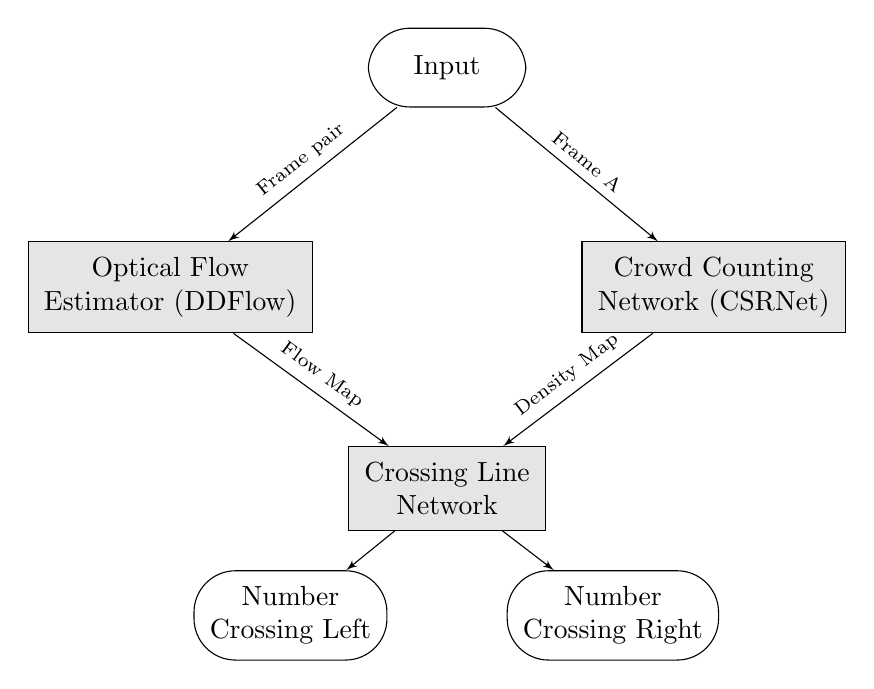
\begin{tikzpicture}[>=latex']
    \tikzset{block/.style= {draw, rectangle, align=center,minimum width=2cm,minimum height=1cm, inner sep=0.2cm, fill=gray!20},
    rblock/.style={draw, shape=rectangle,rounded corners=1.5em,align=center,minimum width=2cm,minimum height=1cm, inner sep=0.2cm},
    }
    \node [rblock]  (start) {Input};
    \node [block, below right =1.7cm and 0.7cm of start] (countnet) {Crowd Counting\\Network (CSRNet)};
    \node [block, below left = 1.7cm and 0.7cm of start] (flownet) {Optical Flow\\Estimator (DDFlow)};
    \node [block, below = 4.3cm of start] (linenet) {Crossing Line\\Network};
    \node [rblock, below right =0.5cm and -0.5cm of linenet] (crossright) {Number\\Crossing Right};
    \node [rblock, below left = 0.5cm and -0.5cm of linenet] (crossleft) {Number\\Crossing Left};
    %% Coordinate on left and middle

% paths
    \path[draw,->, every node/.style={sloped,anchor=south,auto=false, font=\scriptsize}]
                (start) edge node {Frame A} (countnet)
                (start) edge node {Frame pair} (flownet)
                (countnet) edge node {Density Map} (linenet)
                (flownet) edge node {Flow Map} (linenet)
                (linenet) edge (crossright)
                (linenet) edge (crossleft)
                ;
\end{tikzpicture}

\subsubsection{Why unsupervised}
For Crowd Counting there are a lot of datasets available and if new data is provided, it is pretty easy to label these and update the model. For Crowd Direction this is a bit more tricky. Older methods use conventional methods which used handcrafted features which predicted pretty well the direction in situations which were pretty standard, but completely failed in situations which were different from the standard. With the introduction of convolutional neural networks in the field this changed. These made it possible to make vastly more robust filters, but with cost of requiring a lot of labeled data (Because supervised learning). All approaches in the earlier papers had the access to huge amount of labeled data, which made this a suitable solution. In situations with not a lot of available data this makes it a lot harder.
The supervised models for Crowd Direction are largely based on general Flow Estimation models which try to predict all the pixels in a frame. More recently there appear methods to make the supervised Flow Estimation models unsupervised. This makes it possible to accurately predict the direction of pixels without the need for huge amounts of labeled data.


\chapter{Background}
In this chapter a selection of terms is explained which gives a basis to understand the rest of this thesis. This background is created with the assumption that the reader has a basic background in Machine Learning and (Convolutional) Neural Networks.

\todo{Reframe ROI and LOI in the introduction or in the rest of the paper}
\section{Region of Interest}
The Region of Interest problem is a widely studied problem in which the goal is to estimate the amount of pedestrians given a single image. Directly predicting the counted pedestrians given a Neural Network is a hard task, because of the lack of supervision, this would require a large amount of samples to accurately solve this task. All recent State-of-the-Art methods therefore use an intermediate representation to give the model enough supervision to perform Crowd Counting with a low amount of training samples.

In the early days of Crowd Counting several methods have been proposed which use \emph{detection-based} methods to estimate the amount of pedestrians \cite{Dalal2005, Dollar2012} . Several papers were introduced which tried to detect only the head \cite{Subburaman2012} and others tried to focus on general part detection \cite{Wu2007, Lin2010}. These methods rely on individually detecting the pedestrians. This becomes much harder when occlusion of the pedestrians start to happen. This is why the performance of these methods start to degrade when the density of the pedestrians in an image start to increase.

Later papers introduced a \emph{regression-based} solution, which tries to predict the amount of pedestrians in crowd blobs \cite{Chan2009, Idrees2013, zheng_cross-line_2019}. Using SVM or other regressor methods and several features such as the amount of foregrounds pixels of the blob and detected key points the count inside crowd blobs were predicted. Regression based solutions were an improvement over the detection methods, but still lack the capabilities to estimate pedestrians counts in highly occluded areas.

\subsection{Density Map}

\begin{figure}[h]
\centering
\includegraphics[width=1.0\textwidth]{images/example_density_demo}
\caption{Example of generated density map on the right side, for the left image}
\label{fig:density_map}
\end{figure}
With the introduction of Convolutional Neural Networks in the field of Crowd Counting density maps were proposed as well to count pedestrians \cite{Zhang2016, Liu2019, li2018csrnet}. A \emph{density map} (Figure \ref{fig:density_map}) used for Region of Interest is a map which represents the density of pedestrians of each pixel. The density map is generated by taking the locations of each pedestrian ($p=\begin{bmatrix} x_p \\ y_p \end{bmatrix}$ in equation \ref{eq:density_pixel}) and place those locations on the the density map.

Individual dots are very hard for a Neural Network to detect correctly and are proned to errors. To circumvent this a Gaussian shaped circle is created around this location, still with with a sum of 1. The amount of pedestrians in the frame can be extracted from the density map by taking the sum over all the pixels of the density map (Equation \ref{eq:density_sum}, where $D_t(p)$ is the density for location $p=\begin{bmatrix} x_p \\ y_p \end{bmatrix}$ for trainings frame $t$).

\begin{equation}
\label{eq:density_pixel}
	D_t(p) = \frac{1}{2 \pi \sigma_p^2}\sum_{p\in P} e^{\frac{(x_p-x)^2+(y_p-x)^2}{-2 \sigma_p^2}}
\end{equation}

\begin{equation}
	\label{eq:density_sum}
	C_t = \sum_{p\in P} D_t(p)
\end{equation}

Several methods have been presented to optimize the generation of density maps \cite{Zhang2016, li2018csrnet, Wan2019}. For most medium dense frames the difference in methods is minimal. Often in benchmarks with medium dense frames a fixed sigma is used ($\sigma_p=\sigma_i$ in equation \ref{eq:density_pixel}). For highly dense frames the use of different methods can have a difference, especially when the difference in size between close pedestrians and pedestrians in the background is large \cite{li2018csrnet}. In our own preliminary results, this has no effect on our datasets.

\section{Flow Estimation}
The research which is done on the Flow Estimation problem is widely used. Approaches on this topic can be used in a wide range of applications which makes it very interesting. Already in the early 1980's Horn and Schunck \cite{Horn1981} published the first paper which tried to predict flow. Since then lots of different approaches have been published \cite{Memin1998, Bruhn2005, Brox2014}. Long conventional mathematical approaches have ruled the flow estimation field. Later also learnable models were introduced \cite{Pock2008, Wedel2009}.

\begin{figure}[h]
\centering
\includegraphics[width=1.0\textwidth]{images/example_flow_demo}
\caption{Example of generated velocity map on the right side, for the left image}
\label{fig:flow_map}
\end{figure}


Recent papers however make use of Convolutional Neural Network based models \cite{Dosovitskiy2015, ilg_flownet_2016, sun_pwc-net_2018, Ranjan2017, Hui2018}. These models predict pixel-precise velocity maps. The \emph{velocity map} (Figure \ref{fig:flow_map}) is a map which predict per pixel of the frame the amount of movement to another location. In equation \ref{eq:flow_basis}, $V_t(p)$ shows the velocity map as a difference between the location of the pixel in the current frame ($p$) and the location of this pixel in the next frame ($N_t(p)$).

\begin{equation}
\label{eq:flow_basis}
V_t(p) = N_t(p) - \begin{bmatrix} x_{p} \\ y_{p} \end{bmatrix}
\end{equation}

Creating a real world dataset that utilizes the power of pixel-wise flow estimation is very hard \cite{Dosovitskiy2015}. There are no real world devices which could capture both video and create pixel perfect ground-truths to train the flow estimation models on. Most of the flow estimation benchmarks are therefore generated videos. Computer 3D-engines make it possible to generate pixel-perfect flow estimation based on the generated videos in the engine.

However there is a large gap in domain and scene between the generated datasets and real world applications \cite{Liu2008}. Recent supervised papers \cite{Dosovitskiy2015, sun_pwc-net_2018} tend to overfit on these datasets and therefore perform rather poor on real world applications. One promising direction is unsupervised learning \cite{Yu2016, Janai2018, liu_ddflow_2019, liu_selflow_2019}. Early papers only predicted non-occluded pixels \cite{Yu2016, Janai2018}, but recent papers use methods to estimate occluded pixels as well \cite{liu_ddflow_2019, liu_selflow_2019}. Further details about these methods in related work.



\section{Line of Interest}
\begin{figure}[h]
\centering
\includegraphics[width=0.6\textwidth]{images/background_LOI_kopie}
\caption{Example of LOI, red: LOI, blue: LOI area}
\label{fig:loi_example}
\end{figure}

Line of Interest is very similar to Region of Interest. Where Region of Interest is the interest of the amount of people inside the ROI, the Line of Interest is the focus on the amount of pedestrians that cross the specified line during a certain timeframe. This LOI is defined as a single line between two points $p_1$ and $p_2$ (Top and bottom point in figure \ref{fig:loi_example})

With the Line of Interest problem the goal is to give the amount of pedestrians crossing of each side given a set of frames (a pre-captured video or video stream). The output of the prediction should give two numbers $c_1$ and $c_2$ which are the amount of pedestrians crossing from each side.

Only a handful of papers are published about Line of Interest. In the earlier papers \cite{ma_counting_2016, cao_large_2015}, slicing was a widely used approach to estimate the Line of Interest. With slicing a small area, called the LOI area (Blue area in figure \ref{fig:loi_example}), is taken around the LOI. Over a set of consecutive frames each slice of the frame was taken and stitched together into a single image. On the images slow walking pedestrians appear rather wide and fast walking pedestrians shallow. By counting the amount of pedestrians present on the stitched image, the total amount of pedestrians crossing the line can be counted.

The area is defined by all the pixels that have a maximum distance to the LOI of $d$ and can be projected on the LOI. When projected, the pixels fall between $p_1$ and $p_2$.

Recent papers discard this method \cite{leibe_crossing-line_2016, zheng_cross-line_2019}, because it makes it hard to track pedestrian with different speeds and walking in different directions give artifacts which make it hard to track those pedestrians \cite{leibe_crossing-line_2016}. The slicing method is replaced with an actual frame by frame prediction method. Using two consecutive frames the amount of pedestrians crossing the line is measured. These newer methods predict both location and direction of the pedestrian. 

Based on these new papers, the problem of Line of Interest is divided into three separate problems. Locating the pedestrians (Region of Interest), estimate the direction (Flow Estimation) of the pedestrians and combining these two streams of information into the count for Line of Interest. Further details of this approach will be provided in related work.

\chapter{Related Work}
In the following parts we try to explain several key subjects to understand the field of Line of Interest.

\section{Region of Interest}
One of the building blocks of all the information reduction is Crowd Counting/Region of Interest. In low density area's individual object detection, such as YOLO, is a good solution. In high density area's the occlusion by pedestrians makes it hard to detect individual pedestrians. Density Maps still provide the possibility to count the amount of people inside an area, but don't have to deal with the exact locations of the heads, which makes it more robust against errors in the prediction.

In contrast to object detection, it is not possible to identify the full body of the pedestrian in the frames. When using downwards facing camera's, such as high hanging surveillance camera's, the only clearly visible part of a pedestrian is the head. Therefore the labeling of the pedestrians is done by selecting a single point on the head.

An individual point is very hard for a Neural Network to find correctly and is prone to errors. Additionally the exact location of an individual pedestrian are not of high importance, only the total count given a certain region.

Density Maps for Crowd Counting are therefore a solution. Instead of finding individual points in the image, which represent a pedestrian, the points are spread out on the density map, by a Gaussian Distribution, which summed together add up to one.

This method results in a robust method to train an end-to-end model for ROI especially in high density images.

% Show a density map with on the left side image with dots and on the right side the density map.

The density map is always a area with several Gaussians. The method to generate those Gaussian's and their size differ.

- All Gaussians same size
- Gaussians differ in size depending on the density of the pedestrians in the neighbourhood
- Gaussian differs in size based on the angle of the video. Hard to do when there is no access to height/angle.

Good paper to cite for benchmark and why we chose this method
\cite{wang2020nwpu}
\cite{li2018csrnet}



\section{Flow Estimation}
Since the early days of image detection different flow estimation methods are proposed. These methods are very general and can be applied to solve a range of different problems.

One of the most widely used methods is the Lucas-Kanade method (For more details \cite{lucas_kan_nutshell}), which was invented in the 80s. It tries to predict the displacement of a pixel in two consecutive frames using equation (\ref{eq:lucas1}).

\begin{equation} \label{eq:lucas1}
I_x(x, y) \cdot u + I_y(x,y) \cdot v = -I_t(x,y)
\end{equation}

With equation (\ref{eq:lucas1}) the goal is to estimate $(y, v)$ which is the direction of the pixel. $I_x(x, y)$ and $I_y(x, y)$ are the derivative of the intensity in both the $x$ and $y$ direction.$I_t(x, y)$ is the difference in intensity between the two consecutive frames $(b-a)$.

The Lucas-Kanade method is an easy and efficient method to estimate moving object, but it lacks on crucial points. It only incorporates gray scale and doesn't work very well with occluded pixels. (Linear movement? Not sure if NN's assume this as well. Probably not, but doesnt matter in our case)

\subsection{FlowNet}
One of the first good working models for Flow Estimation using a Neural Network based architecture is FlowNet \cite{fischer_flownet_2015} and the architecture is still widely used. (FlowNetV2 \cite{ilg_flownet_2016})

The first usable Flow Estimation using an end-to-end CNN was FlowNet, which is still widely used. The network tries per-pixel prediction which direction the flow is moving. This is done using a deep CNN and at the end a refinement to enlarge the remaining volume into an prediction with the same size as the original input frames. (Upconvolving using the output of several in between stages)

Till then a big problem was the trainability of large end-to-end CNN's and there massive hunger of data. Fischer et al. fixed this by generating a massive synthetic dataset called Flying Chairs. This dataset has more than 22000 image pairs which are build up from Flickr backgrounds and in the front chairs which have move using a random affine transformation.





Several issues with FlowNet were the complete reliability on Neural Networks. Some of the tasks inside the Flow Estimator can efficiently be solved with conventional methods. PWCNet (\cite{sun_pwc-net_2018}) uses a combination of an CNN and some conventional methods. This results in a much smaller network, which results in faster training, additionally the smaller network can handle frames quicker.

One of the issues with CNN based flow estimators is the requirement for pixel level labeling per frame. This results in a huge amount of labeled data required for training. One of the solutions for these problems is the generation of synthetic data which, but these solutions do not scale well to the real world.

A solution for the huge amount of labeled data is unsupervised learning. Both DDFlow \cite{liu_ddflow_2019} and SelFlow \cite{liu_selflow_2019} introduce methods to learn from unlabeled video.

- Video Counting explained: Deep Spatio-Temporal Residual Networks for Citywide Crowd Flows Prediction


\section{Line of Interest}
In the earlier days of Line of Interest the method to estimate was by temporal slicing. In each frame a slice of the image is taken, by taking a slice around the LOI. These slices are stitched together, so a small sequence of frames result in a single image of the stitched slices, temporal sliced image. Based on the image the algorithms try to predict how many pedestrians passed the line in the short sequence.

Ma et al. \cite{ma_counting_2016} first uses crowd segmentation on the sliced image, which results in several crowd segments in the image. Then the algorithm performs normalization on the pedestrians, because of the slicing the faster walking pedestrians appear smaller in the temporal slice image. After this the algorithm performs feature extraction using both global features and local features, which are extracted using local HOG (Histogram of Oriented Gradient) features and a bag-of-words model. This results in a single feature vector per crowd segment. Using a regression function with the features as input, the size of the crowd is predicted. The total pedestrian count of the sliced image is then used to calculate the exact count of people crossing the line between two individual frames. This is done by using several sliced images and solving the problem as a integer programming problem.

During the same time Cao et al. \cite{cao_large_2015} first introduced CNN's in the field of LOI. The paper proposes a model which uses three CNN's which predicts the ins and outs of a individual temporal slice. The first CNN predicts the total amount of people in the temporal slice. The second CNN classifies from which direction people are crossing the line based on the optical flow of the temporal sliced image. The third one predict the ratio of pedestrians crossing during the slice, based on the optical flow. By using the outputs of each network, the algorithm is able to accurately predict the instant count. Additionally Cao et al. \cite{cao_large_2015} shows that the use of CNN's improves the versatility of the models. The model performs better on almost all scenario's and is much more robust with changing weather scenario's and changing angles, than the method of Ma et al. \cite{ma_counting_2016}

Zhao et al. \cite{leibe_crossing-line_2016} introduced a new approach to process the images. Instead of using temporal sliced images. The method directly tries to predict the crowd count based on two consecutive frames. Additionally it merges the Crowd Counting and Crowd Flow models into a single CNN. The paper uses FlowNet as base for the model. Only the last layer predicts both the flow and the crowd density map, as described in Crowd Counting. Additionally the model doesn't try to predict precise direction of every pixel, because the labeled data provided for the model doesn't use pixel precise Flow Estimation. The flow estimator only uses the dot-annotated location of the heads.

Zheng et al. \cite{zheng_cross-line_2019} provides in a era where CNN's have most of the records in hand, a method which scores SOTA on the benchmark for LOI. The model is extremely fast and only uses SVM's and linear regression to end state of the art. Problem with the model, it is very hard to tweak to very dynamic datasets such as the ArenaPeds dataset.



- Explain quickly why we can't just use YOLO (Low density)
-

\chapter{Method}

\section{Instant LOI counting}
In our thesis two method are use to come up with instant LOI counts. Both methods use the same approach, but the region-wise uses the pixel-wise approach on a region-level to improve smoothing of the velocity and density map. This will help when the density map and velocity map don't align correctly.

\subsection{Pixel-level counting}
The proposed method by \cite{leibe_crossing-line_2016} in related work section \ref{section:crossing_line_2016} uses some simplifications. By reframing the pixel-level counting in the following way. The approach is much more theoretical correct.

\label{sec:pixel_level}
We define $v_{perp}$ as the normalized directional vector perpendicular to the LOI (Two solutions are perpendicular on the LOI and this defines sides 1 and 2 of the LOI counting). Then we define the collection of the pixels on the left side of the LOI and inside the LOI area as $M_1$ (side 1) and the pixels on the right side (side 1 and inside the LOI area) as $M_2$.
\todo{Draw picture with LOI area, sets of pixels and vperp}

The velocity towards the LOI is then defined as the dot-product of $V_t$ and $v_{perp}$ (Equation \ref{eq:v_proj}).

\begin{equation}
	Q_t(p) = V_t(p) \cdot v_{perp}
	\label{eq:v_proj}
\end{equation}


\begin{equation}
\begin{aligned}
	c_{1,t} =& \sum_{\{p \in M_1 | Q_t(p) > 0\}} C_t(p) \cdot \frac{Q_t(p)}{d}\\
	c_{2,t} =& \sum_{\{p \in M_2 | Q_t(p) < 0\}} C_t(p) \cdot \frac{-Q_t(p)}{d}
\end{aligned}
\label{eq:pixel_cross}
\end{equation}

Then then the LOI count on timestep $t$ is then defined in equation \ref{eq:pixel_cross}. Where $\frac{Q_t(p)}{d}$ defines the percentage that the density on the specific pixel, has crossed the LOI area. Lastly we can sum the count over a timespan into a single count for each side as in equation \ref{eq:zhao_timeframe_sum}.

\subsection{Region-level counting}
To smooth the velocity around the LOI a new method is proposed. Instead of using the individual pixel velocities for the density map, binning is applied. Several regions have been defined to smooth out the velocity and density. Each region is defined $M_{1,r}$, which is a subset of $M$.

\begin{equation}
	\begin{aligned}
		c_{1,t} =& \sum^R_{r} \frac{\sum_{\{p \in M_{1,r} | Q_t(p) > 0\}} Q_t(p)}
		{d \cdot \sum_{\{p \in M_{1,r} | Q_t(p) > 0\}} 1} \cdot \sum_{\{p \in M_{1,r} | Q_t(p) > 0\}} C_t(p)\\
		c_{2,t} =& \sum^R_{r} \frac{\sum_{\{p \in M_{2,r} | Q_t(p) > 0\}} -Q_t(p)}
		{d \cdot \sum_{\{p \in M_{2,r} | Q_t(p) > 0\}} 1} \cdot \sum_{\{p \in M_{2,r} | Q_t(p) > 0\}} C_t(p)
	\end{aligned}
	\label{eq:region_cross}
\end{equation}

The same setup is applied as in section \ref{sec:pixel_level}, but equation \ref{eq:pixel_cross} is replaced for equation \ref{eq:region_cross}. Where for each region the average velocity is taken (towards the LOI), which is then multiplied with the sum of the density (towards the LOI) inside the region.

\todo{Display a with regions defined LOI}

\subsection{Adaptive LOI area}
How to adaptively estimate the LOI area.
\todo{More thorough seeking in this}


\section{Network}


For our system we split up the program into 3 parts. The Crowd Counting models, the Flow Estimation models and the Line of Interest. The methods which combine the Crowd Counting and the Flow Estimation in a single model are called Crowd Flow models (Useful as directory in the final code)

train.py \# Train the models (All models should be trainable in this file, because they all share the same kind of dataloader)

test.py \# Test the LOI methods using a trained network from train.py (Based on the datasets provided)

run.py \# Run from a video stream live. (Would be super cool and very useful to actual demo this thing)

loi\_models/ (Line of Interest models) - Pixelswise/Regionwise

fe\_models/ (Flow Estimation models) - PWCNet
cc\_models/ (Crowd Counting models) - CSRNet
cf\_models/ (Crowd Flow models) - New Network



\section{Implementation}

\chapter{Datasets}
In this chapter we explain the datasets in more depth. First we explain the requirements of the dataset to correctly train and evaluate each dataset. To compensate for lack of some required labeling a tool is written and explained. Lastly all the datasets are explained in more depth.

\section{Requirements}
For training and evaluation we need two different methods of labeling. For the density map generation the position of each pedestrian is required for the frames which are used for training. For evaluation the line crossing it is required to label the amount of pedestrians crossing the LOI from each side. Ideally the training set is purely labeled with head-tags and the evaluation set only with line crossing labeling.

\section{Labeling}
\begin{figure}[!htb]
\centering
\includegraphics[width=0.6\textwidth]{images/labeler}
\caption{User interface of the labeler}
\label{fig:labeler}
\end{figure}

Several Crowd Counting datasets provide sequences of frames with corresponding pedestrian labeling. However most of those datasets don't provide line crossing labeling. Therefore I build a tool to label videos for line crossing (Figure \ref{fig:labeler}).
The labeler loads a video from the unlabeled videos. In this video the user can label multiple lines by first clicking on the video to draw a line and afterwards fill in the amount of pedestrians crossing the line during the video. Additionally the user can scroll and view through the video using multiple manipulations.


\section{Datasets}
\begin{figure}[h]
\centering
\begin{subfigure}{.33\textwidth}
  \centering
  \includegraphics[width=.8\linewidth]{images/dataset_ucsd}
  \caption{UCSD}
  \label{fig:dataset_ucsd}
\end{subfigure}%
\begin{subfigure}{.33\textwidth}
  \centering
  \includegraphics[width=1.0\linewidth]{images/dataset_fudan}
  \caption{Fudan-ShanghaiTech}
  \label{fig:dataset_fudan}
\end{subfigure}%
\begin{subfigure}{.33\textwidth}
  \centering
  \includegraphics[width=.8\linewidth]{images/dataset_ucsd}
  \caption{AI City Challenge}
  \label{fig:dataset_aicity}
\end{subfigure}%
\caption{Samples of each dataset}
\label{fig:datasets}
\end{figure}

\subsection{UCSD}
The UCSD Pedestrian dataset \cite{Chan2008} is a public dataset created in 2008. The dataset contains a video of a path where people cross each other (See figure \ref{fig:dataset_ucsd}). The dataset is 720x480 in resolution. The original videos are in 30fps, but are downscaled to 10fps. A total of 5680 frames are captured. The first 2000 frames contain line of interest labeling \cite{Ma2013}. Frames 0-599 and 1400-1999 are used for testing. The rest of the frames are used as training samples.

For the training samples all the locations of each pedestrian is provided, so no extra labeling required for density generation \cite{Chan2012}.

\subsection{Fudan-ShanghaiTech}
The Fudan ShanghaiTech dataset \cite{Fang2019} is a public dataset with 100 videos of 13 different scenes. Each video contains 6 seconds of footage at 25 fps and have a resolution of 1920x1080 or 1280x720 (Sample of scene in figure \ref{fig:dataset_fudan}). The scenes have between 20-100 pedestrians per frame. In each frame the pedestrians in the frame are labeled with a bounding-box and a center-point of the bounding-box. The dataset contains 60 training videos and 40 testing videos.

The lack of trajectories and custom line crossing labeling requires the use of the custom build labeler (Figure \ref{fig:labeler}). This is done on the 40 videos of the test set.

\subsection{AI City Challenge}


\chapter{Results}
\section{UCSD}
- Table with Line of Interest

\begin{table}[!htb]
    \begin{minipage}{.5\linewidth}
      \centering
		\begin{tabular}{lll}
		\hline
		Method (ROI)                               & MAE & MSE \\ \hline
		\multicolumn{1}{l|}{CSRNet}          & 0.0 & 0.0 \\
		\multicolumn{1}{l|}{Baseline}        & 0.0 & 0.0 \\
		\multicolumn{1}{l|}{Baseline + flow} & 0.0 & 0.0 \\ \hline
		\end{tabular}
		\caption{\label{tab:roi_ucsd}The ROI results for UCSD}
	\end{minipage}
	\begin{minipage}{.5\linewidth}
      \centering
		\begin{tabular}{lll}
		\hline
		Method (LOI)                               & MAE & MSE \\ \hline
		\multicolumn{1}{l|}{CSRNet + PWCNet}          & 0.0 & 0.0 \\
		\multicolumn{1}{l|}{Baseline}        & 0.0 & 0.0 \\
		\multicolumn{1}{l|}{Baseline + flow} & 0.0 & 0.0 \\ \hline
		\end{tabular}
		\caption{\label{tab:loi_ucsd}The LOI results for UCSD}
	\end{minipage}
\end{table}

\section{CrowdFlow}

\begin{table}[!htb]
    \begin{minipage}{.5\linewidth}
      \centering
		\begin{tabular}{lll}
		\hline
		Method (ROI)                               & MAE & MSE \\ \hline
		\multicolumn{1}{l|}{CSRNet}          & 0.0 & 0.0 \\
		\multicolumn{1}{l|}{Baseline}        & 0.0 & 0.0 \\
		\multicolumn{1}{l|}{Baseline + flow} & 0.0 & 0.0 \\ \hline
		\end{tabular}
		\caption{\label{tab:roi_crowdflow}The ROI results for CrowdFlow}
	\end{minipage}
	\begin{minipage}{.5\linewidth}
      \centering
		\begin{tabular}{lll}
		\hline
		Method (LOI)                               & MAE & MSE \\ \hline
		\multicolumn{1}{l|}{CSRNet + PWCNet}          & 0.0 & 0.0 \\
		\multicolumn{1}{l|}{Baseline}        & 0.0 & 0.0 \\
		\multicolumn{1}{l|}{Baseline + flow} & 0.0 & 0.0 \\ \hline
		\end{tabular}
		\caption{\label{tab:loi_crowdflow}The LOI results for CrowdFlow}
	\end{minipage}
\end{table}

\section{Fudan-ShanghaiTech}

\begin{table}[!htb]
    \begin{minipage}{.5\linewidth}
      \centering
		\begin{tabular}{lll}
		\hline
		Method (ROI)                               & MAE & MSE \\ \hline
		\multicolumn{1}{l|}{CSRNet}          & 0.0 & 0.0 \\
		\multicolumn{1}{l|}{Baseline}        & 0.0 & 0.0 \\
		\multicolumn{1}{l|}{Baseline + flow} & 0.0 & 0.0 \\ \hline
		\end{tabular}
		\caption{\label{tab:roi_fudan}The ROI results for Fudan}
	\end{minipage}
	\begin{minipage}{.5\linewidth}
      \centering
		\begin{tabular}{lll}
		\hline
		Method (LOI)                               & MAE & MSE \\ \hline
		\multicolumn{1}{l|}{CSRNet + PWCNet}          & 0.0 & 0.0 \\
		\multicolumn{1}{l|}{Baseline}        & 0.0 & 0.0 \\
		\multicolumn{1}{l|}{Baseline + flow} & 0.0 & 0.0 \\ \hline
		\end{tabular}
		\caption{\label{tab:loi_fudan}The LOI results for Fudan}
	\end{minipage}
\end{table}


\begin{table}[]
\begin{minipage}{.5\linewidth}
\centering
\begin{tabular}{ll}
\hline
Method                             & FPS \\ \hline
\multicolumn{1}{l|}{CSRNet+PWC}    & 0.0 \\
\multicolumn{1}{l|}{CSRNet+PWC+optimized}& 0.0 \\
\multicolumn{1}{l|}{Baseline}      & 0.0 \\
\multicolumn{1}{l|}{Baseline+flow} & 0.0 \\
\multicolumn{1}{l|}{Baseline+flow+optimized} & 0.0 \\ \hline
\end{tabular}
\caption{\label{tab:fps_fudan}Processing speed}
\end{minipage} %
\begin{minipage}{.5\linewidth}
\centering
\begin{tabular}{lll}
		\hline
		FPS                               & MAE & MSE \\ \hline
		\multicolumn{1}{l|}{25}          & 0.0 & 0.0 \\
		\multicolumn{1}{l|}{12.5}        & 0.0 & 0.0 \\
		\multicolumn{1}{l|}{8.3}        & 0.0 & 0.0 \\
		\multicolumn{1}{l|}{5}        & 0.0 & 0.0 \\
		\multicolumn{1}{l|}{2.5} & 0.0 & 0.0 \\ \hline
		\end{tabular}
\caption{\label{tab:fps_fudan} Optimal FPS}
\end{minipage}
\end{table}

\section{ArenaPeds}
\begin{table}[!htb]
    \begin{minipage}{.5\linewidth}
      \centering
		\begin{tabular}{lll}
		\hline
		Method (ROI)                               & MAE & MSE \\ \hline
		\multicolumn{1}{l|}{CSRNet}          & 0.0 & 0.0 \\
		\multicolumn{1}{l|}{Baseline}        & 0.0 & 0.0 \\
		\multicolumn{1}{l|}{Baseline + flow} & 0.0 & 0.0 \\ \hline
		\end{tabular}
		\caption{\label{tab:roi_fudan}The ROI results for ArenaPeds}
	\end{minipage}
	\begin{minipage}{.5\linewidth}
      \centering
		\begin{tabular}{lll}
		\hline
		Method (LOI)                               & MAE & MSE \\ \hline
		\multicolumn{1}{l|}{CSRNet + PWCNet}          & 0.0 & 0.0 \\
		\multicolumn{1}{l|}{Baseline}        & 0.0 & 0.0 \\
		\multicolumn{1}{l|}{Baseline + flow} & 0.0 & 0.0 \\ \hline
		\end{tabular}
		\caption{\label{tab:loi_fudan}The LOI results for ArenaPeds}
	\end{minipage}
\end{table}


\begin{table}[]
\begin{minipage}{.5\linewidth}
\centering
\begin{tabular}{ll}
\hline
Method                             & FPS \\ \hline
\multicolumn{1}{l|}{CSRNet+PWC}    & 0.0 \\
\multicolumn{1}{l|}{CSRNet+PWC+optimized}& 0.0 \\
\multicolumn{1}{l|}{Baseline}      & 0.0 \\
\multicolumn{1}{l|}{Baseline+flow} & 0.0 \\
\multicolumn{1}{l|}{Baseline+flow+optimized} & 0.0 \\ \hline
\end{tabular}
\caption{\label{tab:fps_fudan}Processing speed}
\end{minipage} %
\begin{minipage}{.5\linewidth}
\centering
\begin{tabular}{lll}
		\hline
		FPS                               & MAE & MSE \\ \hline
		\multicolumn{1}{l|}{25}          & 0.0 & 0.0 \\
		\multicolumn{1}{l|}{12.5}        & 0.0 & 0.0 \\
		\multicolumn{1}{l|}{8.3}        & 0.0 & 0.0 \\
		\multicolumn{1}{l|}{5}        & 0.0 & 0.0 \\
		\multicolumn{1}{l|}{2.5} & 0.0 & 0.0 \\ \hline
		\end{tabular}
\caption{\label{tab:fps_fudan} Optimal FPS}
\end{minipage}
\end{table}

\section{Flow estimation impact}
Qualitative comparison

\chapter{Conclusion}
In this thesis we have shown several points. Crowd Crossing Counting is possible without the supervised knowledge of the Flow Estimation. Two new models are proposed with which the flow enhanced model outperforms the strong baseline which suggests that knowledge about the flow improves the density map prediction for moving objects.

Additionally we have shown both quantitive and qualitative that the maxing filter is an effective method to realign the flow map and the density map, which drastically increases the performance.

Lastly we did a thorough analysis on real world performance. According to the results it would be possible to run the model real time on a fast GPU without optimization. Further optimization could lead to an even quicker model.


\section{Further research}
Due to the lack of high density videos, the full potential of this network can't be shown to its full extend. For further research it would be ideal to propose such a high density map.

\bibliographystyle{apalike}
\bibliography{all}

\appendix
\chapter{Appendix}

\begin{figure}[h]
\centering
\includegraphics[width=0.8\textwidth]{images/proposed_decoder}
\caption{Full decoder for density prediction}
\label{fig:unified_proposed_model}
\end{figure}


\end{document}
